\def\GelfandCanonicalInclusionCaption{кан.\\вкл.}
\begin{center}
\begin{minipage}[t]{.46\linewidth}\vspace{0pt}\centering
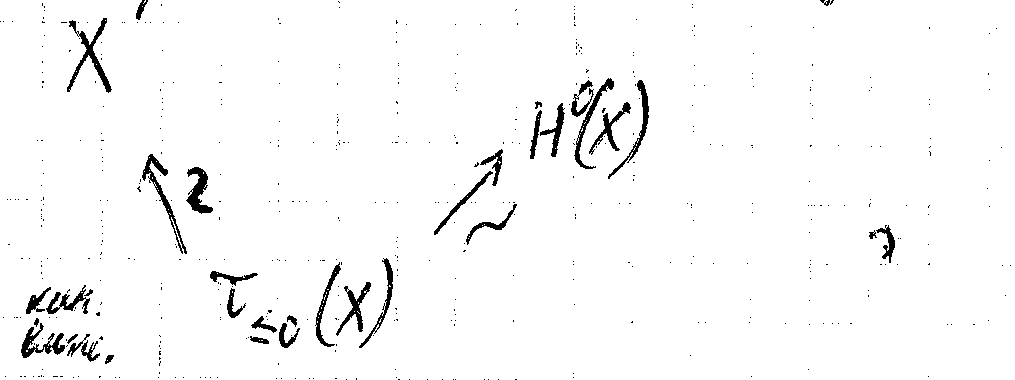
\includegraphics[width=\linewidth]{figures/gelfand-0152-p001396-truncation-original-r2.png}\par\smallskip
{\footnotesize Оригинал рукописного рисунка: \texttt{GELFAND-P001396}}
\end{minipage}\hfill
\begin{minipage}[t]{.50\linewidth}\vspace{0pt}\centering
{\footnotesize Частичное воссоздание видимых штрихов}\par\smallskip
% Requires the language-local caption macro \GelfandCanonicalInclusionCaption.
% The label on the left remains a candidate list, not a selected reading.
\begin{tikzpicture}[x=.88cm,y=.88cm,line width=.55pt,>=stealth]
\node at (0,1.55) {$X$};
\node at (3.08,1.05) {$H^0(X)$};
\node at (1.02,-.30) {$\tau_{\le0}(X)$};
\draw[->] (.58,.04)--(.05,.92);
\draw[->] (1.92,.14)--(2.68,.89);
\node[font=\scriptsize] at (.93,.64) {$\sim/2/\iota$?};
\node at (2.39,.26) {$\sim$};
\node[font=\scriptsize,align=center] at (-.18,-.33) {\GelfandCanonicalInclusionCaption};
% The isolated right-hand ink stroke has no assigned mathematical meaning.
\draw (4.08,.20) .. controls (4.25,.44) and (4.34,.16) .. (4.22,.08)
  .. controls (4.16,.02) and (4.30,.13) .. (4.26,.22);
\end{tikzpicture}

\end{minipage}
\end{center}
\noindent{\small\textit{Подпись левой стрелки остаётся среди кандидатов: тильда,2,йота. Квазиизоморфность в данном примере не определяет начертание знака. Отдельный правый штрих сохранён без толкования.}}
